\documentclass[12pt]{article}

\usepackage{graphicx}
\usepackage{caption}
\usepackage{amssymb,amsmath,amsthm}




% the following commands set the size of printed page
\setlength{\textheight}{680pt} \setlength{\topmargin}{-50pt}
\setlength{\textwidth}{500pt}
\setlength{\evensidemargin}{-10pt}
\setlength{\oddsidemargin}{-10pt}
%%%%%%%%%%%%%%%%%%%%%%%%%%%%

\begin{document}

\title{Place title of Group Project Here}
\author{Riley Davidson, Laren Edwards, Dallan Olsen, Calix Barrus}

%% comment out next command to put today's date after names of group members, or put a desired day in the parethesis
\date{}

\maketitle

\begin{abstract}
Place Abstract Here.
\end{abstract}

%% First Section
\section{Background/Movitation}
Put your background motivation stuff here. You might reference something material here like \cite{ref1}.

%% Second Section 
\section{Modeling PDE for Traffic Flow}

To begin our first foray into modelling traffic flow, we will pull from Volume 4 and work with the given equation for traffic flow $u_t + V_\infty \left(1 - \frac{2u}{u_{\infty}} \right) u_x = 0$. We want to consider three cases:
\begin{enumerate}
    \item What happens to the left of a light after a red light turns green?
    \item What happens before a light when a light turns from green to red? 
    \item What happens both before and after a light when it turns from red to green?
\end{enumerate}

\subsection{Method of Characteristics} 
To begin, we will try to find an explicit solution using the method of characteristics. 

Suppose the solution $u$ is some curve parameterized by $s$ as $u(x(s), t(s))$. Taking the derivative of $u$ with respect to $s$ gives 
\begin{align*} % in the book, the start off with the claim that this equation is = 0 or = f. How do we justify setting u' equal to the differential equation, and also equal to the RHS of the PDE? 
    u'(x(s), t(s)) = \frac{\partial u}{\partial x} \frac{\partial x}{\partial s}  + \frac{\partial u}{\partial t} \frac{\partial t}{\partial s} = u_x \frac{\partial x}{\partial s}  + u_t \frac{\partial t}{\partial s}
\end{align*}
and matching terms with the original differential equation gives us that 
\begin{align*}
    \frac{\partial x}{\partial s}  = V_\infty \left( 1 - \frac{2}{u_\infty} u \right) \\
    \frac{\partial t}{\partial s} = 1 \\
    \frac{\partial u}{\partial s} = 0 .
\end{align*}

Using the fact that $\frac{\partial t}{\partial s} = 1$, we have that 
\begin{align*}
    \frac{\partial x }{\partial t} = V_\infty (1 - \frac{2}{u_\infty} ) \\
    x(t) - x(0) = \int_{0}^{t} V_\infty(1 - \frac{2}{u_\infty} u) dt \\
    x = V_\infty(1 - \frac{2}{u_\infty} u) t + x(0) \\
    t = \frac{1}{  V_\infty(1 - \frac{2}{u_\infty} u) }x - x(0)
\end{align*}
where to evaluate the integral, we used the fact that $\frac{\partial u}{\partial s}$ is $0$, and so the characteristics are constant along the plane. This yields a few cases for the characterstic curves depending on what value of $u$ the curve takes. Based on the physical properties of our model, we have that $u \in [0, u_\infty]$. The slope of the characteristics changed depending on the value of $u$, specifically the slope $m = > 0$ when $u \in [0, \frac{u_\infty}{2}) $, the slope is vertical or undefined when $u = \frac{u_\infty}{2}$, and $m < 0$ when $u \in ( \frac{u_\infty}{2}, u_\infty]$.

Next, suppose that there are some values $x_0, x_1$ from which we draw characteristic curves, and suppose $u(x_0) < u(x_1)$. This will result in shocks, (assuming the shocks happen inside the domain of relevance). See Figures \ref{fig:shock_x1_x2_lt_half}, \ref{fig:shock_x1_x2_gt_half}, and \ref{fig:shock_x1_eq_half} for examples. 

\begin{figure}[!htb]
    \captionsetup{justification=centering}
    \minipage{0.32\textwidth}
    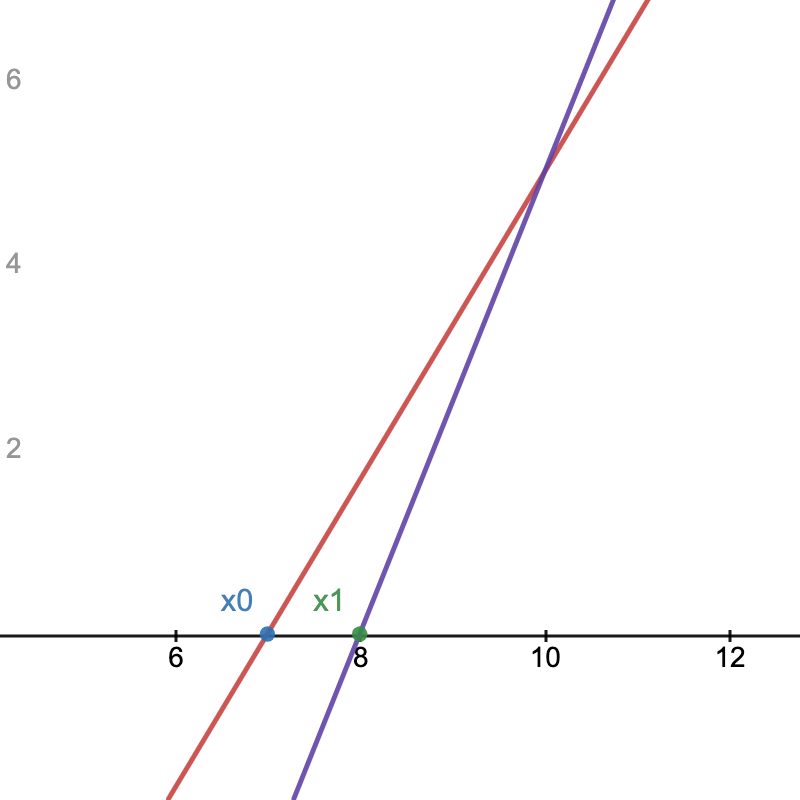
\includegraphics[width=\linewidth]{shock_x1_x2_lt_half.png}
    \caption{$u(x_0) < u(x_1), u(x_0), u(x_1) \in (0, \frac{u_\infty}{2})$}\label{fig:shock_x1_x2_lt_half}
    \endminipage\hfill
    \minipage{0.32\textwidth}
    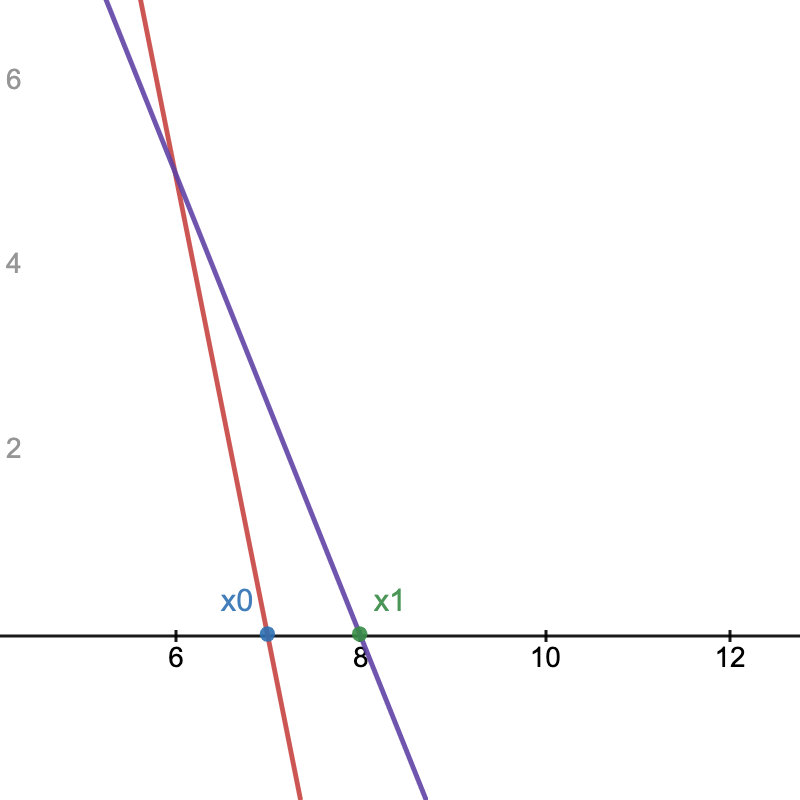
\includegraphics[width=\linewidth]{shock_x1_x2_gt_half.png}
    \caption{$u(x_0) < u(x_1), u(x_0), u(x_1) \in (\frac{u_\infty}{2}, u_\infty)$}\label{fig:shock_x1_x2_gt_half}
    \endminipage\hfill
    \minipage{0.32\textwidth}%
    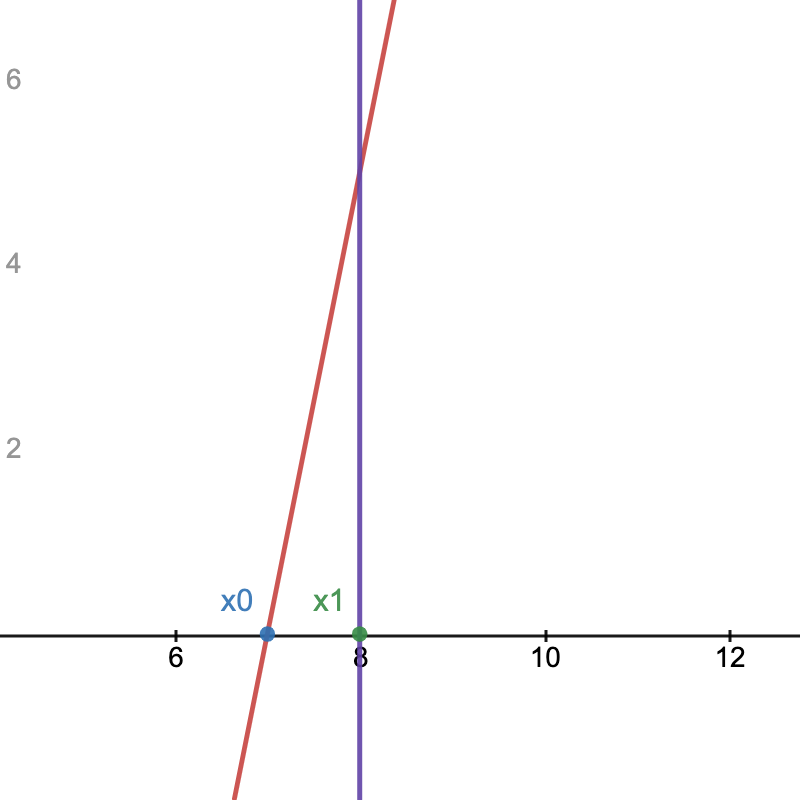
\includegraphics[width=\linewidth]{shock_x1_eq_half.png}
    \caption{$u(x_0) < u(x_1), u(x_0) \in (\frac{u_\infty}{2}, u_\infty), u(x_1) = \frac{u_\infty}{2} $}\label{fig:shock_x1_eq_half}
    \endminipage
\end{figure}

Conversely, if the density of the initial condition is decreasing (i.e. when $x_0 < x_1 \implies u(x_0) < u(x_1)$), there are no shocks. See Figure 

\begin{figure}[!htb]
    \captionsetup{justification=centering}
    \minipage{0.32\textwidth}
    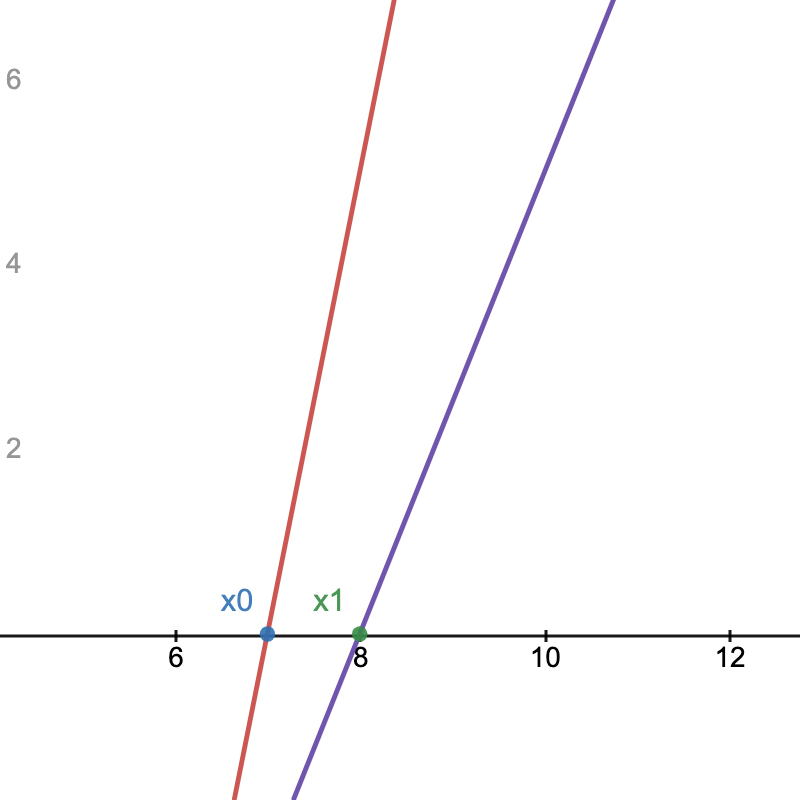
\includegraphics[width=\linewidth]{no_shock_x1_x2_lt_half.png}
    \caption{$u(x_0) > u(x_1), u(x_0), u(x_1) \in (0, \frac{u_\infty}{2})$}\label{fig:no_shock_x1_x2_lt_half}
    \endminipage\hfill
    \minipage{0.32\textwidth}
    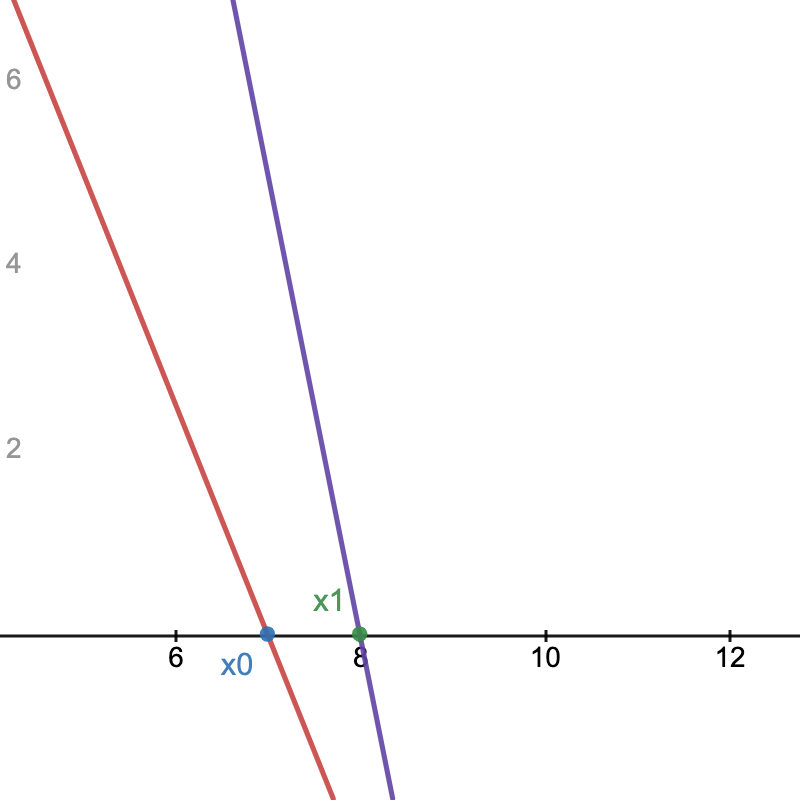
\includegraphics[width=\linewidth]{no_shock_x1_x2_gt_half.png}
    \caption{$u(x_0) > u(x_1), u(x_0), u(x_1) \in (\frac{u_\infty}{2}, u_\infty)$}\label{fig:no_shock_x1_x2_gt_half}
    \endminipage\hfill
    \minipage{0.32\textwidth}%
    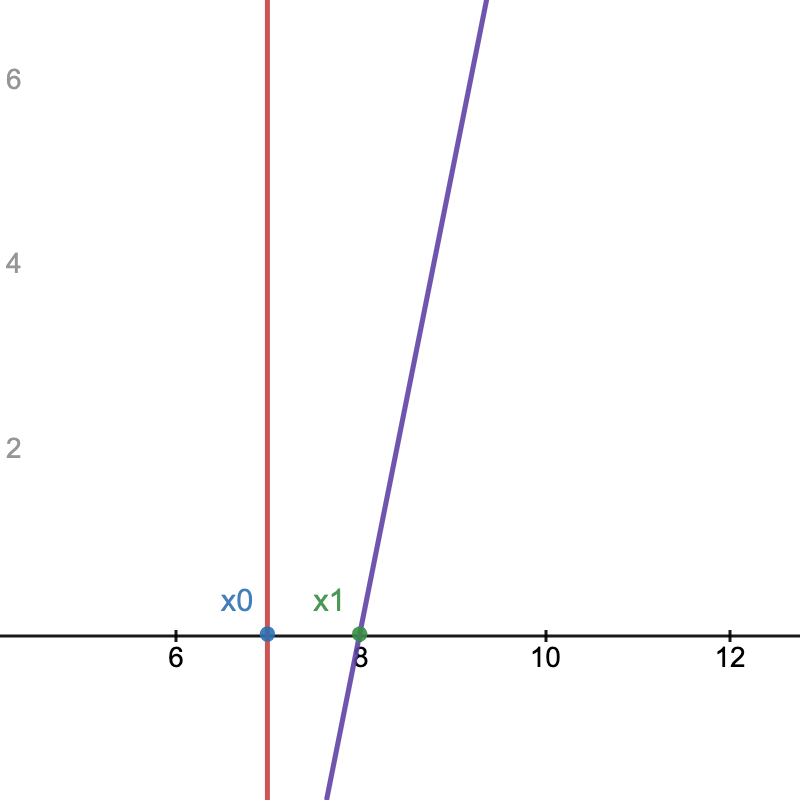
\includegraphics[width=\linewidth]{no_shock_x0_eq_half.png}
    \caption{$u(x_0) < u(x_1), u(x_0) = \frac{u_\infty}{2},  u(x_0) \in (\frac{u_\infty}{2}, u_\infty) $}\label{fig:no_shock_x0_eq_half}
    \endminipage
\end{figure}

Write up numerical scheme with boundary conditions
Try to figure out why sheme is unstable
Apply to scenarios
Note instability
Try extending domain horizontally with an unrealistic rhs boundary condition OR have the cars come to red light (neumann)
Figure out code for neumann b.c.

try case 2 (will need to knock out diffusion term)

combine simulations for case 3, TEEEHEHEEEEEEEEEEh

Get this on overleaf
Get riley and Laren's stuff  on here 

\begin{verbatim}
This stuff looks like code
            Tabs show up!
\end{verbatim}


%% Third Section
\section{Results/Analysis}

\section{Modeling using SIR Model Type ODEs}

\section{Results/Analysis}

%%Fourth Section
\section{Conclusions}

\begin{thebibliography}{99}
\bibitem{ref1} First reference goes here
\end{thebibliography}

\end{document}
